%----------------------------------------------------------------------------------------------
%----------------------------------     2. Taylor-Theorie    ----------------------------------
%----------------------------------------------------------------------------------------------
\section{Taylor-Theorie}

%----------------------------------------------------------------------------------------------
%-----------------------------------     2.1 Taylor-Reihe    ----------------------------------
%----------------------------------------------------------------------------------------------
\subsection{Taylor-Reihe (Approximation höherer Ordnung)}

\begin{tabular}{ll}
    $n$             & Ordnung der Approximationsfunktion $p_n(x)$ \\
    $h = x - x_0$   & Abstand zum Entwicklungspunkt
\end{tabular}

\renewcommand{\arraystretch}{2.3}
\begin{tabular}{l}
    $p_n(x) = f(x_0) + \overbrace{f'(x_0)\cdot h}^{\text{1. Ordnung}} + \overbrace{\frac{f''(x_0)}{2!} \cdot h^2}^{\text{2. Ordnung}} + ... + \overbrace{\frac{f^{(n)}(x_0)}{n!} \cdot h^n}^{n. \text{ Ordnung}}$  \\ 
    $p_n(x) = \sum\limits_{k=0}^{n} \frac{f^{(k)}(x_0)}{k!} \cdot h^k \; \Big|_{h = x-x_0}$ 
\end{tabular}
\renewcommand{\arraystretch}{1}

\vspace{0.2cm}
Der Approximationsfehler $R_n (x_0, h)$ entspricht $f(x) - p_n(x)$ und wird im nächsten Abschnitt beschrieben.		

%----------------------------------------------------------------------------------------------
%-----------------------------------     2.2 Taylor-Reihe    ----------------------------------
%----------------------------------------------------------------------------------------------
\subsection[Fehler Rn der Taylor-Reihe]{Fehler $R_n$ der Taylor-Reihe}

Der Fehler ist nicht klar berechenbar, sondern nur auf einem Intervall "bestimmbar" \\
\textrightarrow\ Worst Case!	

Voraussetzung: $f$ auf Intervall [$a;b$] mind. $(n+1)$ mal ableitbar
\vspace{0.2cm}

\begin{tabular}{ll}
    \textbf{Lagrange:}  &  $\vert R_n \vert = \Big| \frac{f^{(n+1)}(\xi)}{(n+1)!} \cdot h^{n+1} \Big| $ \\
    \\
    \textbf{Cauchy:}    & $\vert R_n \vert = \Big| \frac{f^{(n+1)} (\xi)}{n!}  \cdot h^{n+1} \cdot (1 - \theta)^n \Big|$ \\
    \\
                        & $0 < \theta < 1$    $\xi = x_0 + \theta \cdot h$ \\
                        & $\theta$ steuert Lage von $\xi$ auf Intervall \\
\end{tabular}


\begin{center}
    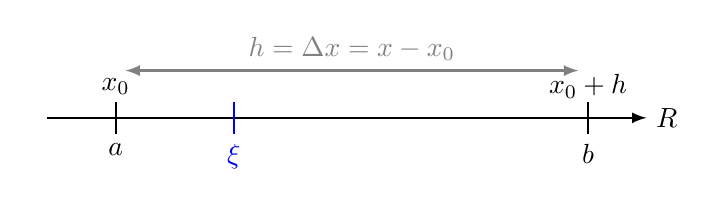
\begin{tikzpicture}
        [
            scale=1.0,
            >=latex
        ]
    
        % nodes
        \node               at (0, 0)   (O) {};             % Ursprung
        \node               at (8, 0)   (H) {$\mathbb{R}$}; % Pfeil-Ende
        \node               at (1, 0.6) (A) {};
        \node               at (7, 0.6) (B) {};
        \node               at (1, 0.4) (x0) {$x_0$};
        \node               at (7, 0.4) (x0h) {$x_0 + h$};

        % lines
        \draw[->, thick]            (O) -- (H);
    
        \draw[thick]            (1, 0.2) -- (1, -0.2) node[below] (a) {$a$};
        \draw[thick]            (7, 0.2) -- (7, -0.2) node[below] (b) {$b$};
        \draw[thick, blue]      (2.5, 0.2) -- (2.5, -0.2) node[below] (xi) {$\xi$};
    
        \draw[<->, thick, gray] (A) to node[above] {$h = \Delta x = x - x_0$} (B);
    \end{tikzpicture}
\end{center}


